\documentclass{article}

% Language setting
\usepackage[english]{babel}
\setlength{\parindent}{0pt}

% Useful packages
\usepackage{booktabs}
\usepackage{array}
\usepackage{amsmath}
\usepackage{graphicx}
\usepackage{float}
\usepackage[colorlinks=true, allcolors=blue]{hyperref}
\usepackage[most]{tcolorbox}
\usepackage{ragged2e}

% Fonts
\usepackage[scaled]{helvet}
\renewcommand{\familydefault}{\sfdefault}
\newcolumntype{L}[1]{>{\raggedright\arraybackslash}p{#1}}
\newcolumntype{C}[1]{>{\centering\arraybackslash}p{#1}}
\usepackage{pdflscape}
\usepackage{lipsum}
\usepackage{longtable}
\usepackage{caption}
\usepackage{multirow}
\usepackage{tocloft}
\usepackage{mhchem}
\usepackage{etoc}
\usepackage{docmute}

% Geometry
\usepackage[
  a4paper,
  top=1.5in,
  bottom=1in,
  left=1in,
  right=1in,
  headheight=60pt,
  headsep=20pt
]{geometry}

% Define header and footer styles
\usepackage{fancyhdr}
\usepackage{rotating}
\pagestyle{fancy}
\fancyhf{}
\renewcommand{\headrulewidth}{0pt}
\fancyhead[C]{%
    \vspace{25pt}%
  \raisebox{15pt}[0pt][0pt]{%
    \makebox[\textwidth]{%
      
\includegraphics[height=40pt]{resources/rufas.png}\hfill
      \textbf{\today}%
    }%
  }\\[-25pt]
  \centering\textbf{Scientific Documentation of RuFaS Model} \\
  \rule{\textwidth}{1pt}
}

\renewcommand{\footrulewidth}{0.4pt}
\fancyfoot[L]{%
  \begin{tabular}[t]{@{}l@{}}
    Ruminant Farm System\\
    Sci Doc v.1
  \end{tabular}%
}
\fancyfoot[C]{\thepage}
\fancyfoot[R]{%
  \begin{tabular}[t]{@{}r@{}}
    \nouppercase{\leftmark}\\
  \end{tabular}%
}
\fancypagestyle{landscapeplain}{
  \fancyhf{}
  \renewcommand{\headrulewidth}{0pt}
  \renewcommand{\footrulewidth}{0pt}
}

% Bibliography setup
\usepackage[
  backend=biber,
  style=authoryear,
  natbib=true
]{biblatex}

\addbibresource{rufas.bib}

\usepackage{titlesec}
\usepackage{etoolbox}

% Reset subsection counter at each new section
\pretocmd{\section}{\setcounter{subsection}{0}}{}{}

% Roman for \section, Alpha for \subsection, alpha for \subsubsection
\renewcommand{\thesection}{\Roman{section}.}
\renewcommand{\thesubsection}{\Alph{subsection}.}
\renewcommand{\thesubsubsection}{\alph{subsubsection}.}

% --- Title Formats (in size order) ---
\titleformat{\section}
  {\Large\bfseries}
  {\thesection}
  {1em}
  {}

\titleformat{\subsection}
  {\normalsize\bfseries}
  {\thesubsection}
  {1em}
  {}

\titleformat{\subsubsection}
  {\normalsize\bfseries}
  {\thesubsubsection}
  {1em}
  {}

% --- Spacing for each level ---
\titlespacing*{\section}{0pt}{1.5\baselineskip}{1\baselineskip}
\titlespacing*{\subsection}{0pt}{1\baselineskip}{0.5\baselineskip}
\titlespacing*{\subsubsection}{0pt}{0.75\baselineskip}{0.35\baselineskip}

\begin{document}

\include{animal}
\include{manure}
\include{crop_and_soil}
\documentclass{article}

% Language setting
\usepackage[english]{babel}
\setlength{\parindent}{0pt}

% Useful packages
\usepackage{booktabs}  % For better looking tables
\usepackage{array}     % More control over column formatting
\usepackage{amsmath}
\usepackage{graphicx}
\usepackage{float} % Allows strict image placement
\usepackage[colorlinks=true, allcolors=blue]{hyperref}% hyperref makes the TOC clickable
\usepackage[most]{tcolorbox}
% Fonts
\usepackage[scaled]{helvet}
\renewcommand{\familydefault}{\sfdefault}
\newcolumntype{L}[1]{>{\raggedright\arraybackslash}p{#1}}
\newcolumntype{C}[1]{>{\centering\arraybackslash}p{#1}}
\usepackage{pdflscape}  % or \usepackage{lscape}
\usepackage{lipsum} % for dummy text
\usepackage{longtable}
\usepackage{caption}
\usepackage{multirow}
\usepackage{mhchem}


% Geometry
\usepackage[
  a4paper,
  top=1.5in,
  bottom=1in,
  left=1in,
  right=1in,
  headheight=60pt,  % This must match the vertical space used
  headsep=20pt
]{geometry}

% Define header and footer styles
% Fancy Header
\usepackage{fancyhdr}
\usepackage{rotating}
\usepackage{tablefootnote}
\pagestyle{fancy}
\fancyhf{}  % clear all header/footer fields
\renewcommand{\headrulewidth}{0pt}  % no horizontal line
% Header setup
\fancyhead[C]{%
    \vspace{25pt}
  \raisebox{15pt}[0pt][0pt]{%
    \makebox[\textwidth]{%
      
\includegraphics[height=40pt]{resources/rufas.png}\hfill
      \textbf{\today}%
    }
  }\\[-25pt]
  \centering\textbf{Scientific Documentation of RuFaS Model} \\
  \rule{\textwidth}{1pt}
}

\renewcommand{\sectionmark}[1]{\markboth{\thesection~#1}{}}
% Footer setup with a divider line and two lines of text on left and right
\renewcommand{\footrulewidth}{0.4pt}
\fancyfoot[L]{%
  \begin{tabular}[t]{@{}l@{}}
    Ruminant Farm System\\
    Sci Doc v.1
  \end{tabular}%
}
\fancyfoot[C]{\thepage} % Center: page number
\fancyfoot[R]{%
  \begin{tabular}[t]{@{}r@{}}
    \nouppercase{\leftmark}\\ % This pulls in the current section title
  \end{tabular}%
}
% Landscape pages should be blank (no headers/footers)
\fancypagestyle{landscapeplain}{
  \fancyhf{} % clear all
  \renewcommand{\headrulewidth}{0pt}
  \renewcommand{\footrulewidth}{0pt}
}

\usepackage[utf8]{inputenc} % Ensure you're using UTF-8 encoding
% Bibliography setup
\usepackage[
  backend=biber,
  style=authoryear,  % You can change this to numeric, apa, etc.
  natbib=true         % Enables \citep, \citet if desired
]{biblatex}

\addbibresource{resources/feed_storage.bib}  % Your .bib file name
\usepackage{titlesec}
\usepackage{etoolbox}

% Reset subsection counter at each new section
\pretocmd{\section}{\setcounter{subsection}{0}}{}{}

% Roman for \section, Alpha for \subsection, alpha for \subsubsection
\renewcommand{\thesection}{\Roman{section}.}           % I, II, III...
\renewcommand{\thesubsection}{\Alph{subsection}.}       % A, B, C...
\renewcommand{\thesubsubsection}{\alph{subsubsection}.} % a, b, c...

% --- Title Formats (in size order) ---
\titleformat{\section}
  {\Large\bfseries}   % Section: largest
  {\thesection}       % Label
  {1em}               % Spacing between label and title
  {}                  % Before-code

\titleformat{\subsection}
  {\normalsize\bfseries}   % Subsection: medium
  {\thesubsection}
  {1em}
  {}

\titleformat{\subsubsection}
  {\normalsize\bfseries}  % Subsubsection: smallest
  {\thesubsubsection}
  {1em}
  {}

% --- Spacing for each level ---
\titlespacing{\section}{0pt}{10pt plus 2pt minus 1pt}{5pt}
\titlespacing{\subsection}{0pt}{8pt plus 1pt minus 1pt}{4pt}
\titlespacing{\subsubsection}{0pt}{6pt plus 1pt minus 1pt}{3pt}

% Optional: Keep your TOC control if needed
\usepackage{etoc}

% Optional: If using headers/footers
\renewcommand{\sectionmark}[1]{\markboth{#1}{}}

% Remove default date from title
\date{} % Prevents date from appearing in \maketitle


% Define title
\title{\textbf{}}
\author{ }
\setlength{\topskip}{10pt}  % Ensures LaTeX reserves room above the first line
%\usepackage{showframe}

\begin{document}

% Custom Title Page
\begin{titlepage}
  \thispagestyle{empty}
  \centering
  \vspace*{2cm}

  {\Huge\bfseries Ruminant Farm System Model\par}
  \vspace{1cm}

  {\Large Feed Storage Module\par}
  \vspace{1cm}

  {\large \today\par}
  \vspace{1.5cm} % Add space before the image

  
\includegraphics[width=0.25\textwidth]{resources/feed.png} % Adjust size and filename

  \vfill

  {\small v.1; Updated 2026\par}
  \vspace*{1cm}
\end{titlepage}

% Continue with front matter (e.g., table of contents)
\thispagestyle{fancy} % Ensure the header/footer appears on the first page

% Global Table of Contents
\thispagestyle{fancy}
\tableofcontents
\newpage

\listoffigures
\newpage

\listoftables
\newpage

\newpage
\section{Preface: A Day in the Life on a RuFaS Farm}

This document provides a high-level overview of the daily operations of a ruminant farm, as modeled by RuFaS. The overview will be through the eyes of Dr. Rue Fas. One day, Dr. Rue woke up and decided the life of a computer scientist wasn’t for her. So she bought a dairy farm, and this is how she operates it every day.

\paragraph{Feeding the Animals}
Second thing in the morning, after coffee, Dr. Rue checks the calendar to see if it’s time to formulate a new ration for her animals.
\vspace{0.2cm}

If a new ration needs to be formulated, Dr. Rue heads over to the barn where she keeps all her forages and feed. While there, she checks how well all the forages are holding up. After considering the feeds available, the quality of each one, and how much each one costs, she decides on how productive she wants her animals to be. It is a difficult balancing act, but eventually a ration recipe is found that will keep the animals happy while keeping costs low and sustainability high until the calendar says the ration recipe needs to be reformulated.
\vspace{0.2cm}

When Dr. Rue doesn’t need to formulate a new ration, she takes the last ration recipe she made and grabs all the feed and forage the animals need for the day out of the feed barn. If there isn’t enough for the animals, then a new ration is formulated using the steps above.

\paragraph{Taking Care of the Animals}
After making sure all the animals’ feed is taken care of, Dr. Rue moves on to taking care of all the other animal tasks. This includes milking the animals, making sure they’re healthy, getting them pregnant, and numerous other tasks. 
\vspace{0.2cm}

As dawn breaks on the RuFaS farm, the animals awaken after a restful night. Joe, the farm master, prepares a large whiteboard to track HerdReproductionStatistics, ensuring he has all the data he needs for the day’s activities.

\textit{Daily Routine} - After leaving their pens, each animal lines up in front of the barn. Julie, the diligent farm veterinarian, examines them one by one. This daily check includes updates on the following areas:
\begin{itemize}
    \item Nutrients: Each animal begins its day with a quick phosphorus requirement assessment. Julie records these details and updates the animal’s phosphorus-related metrics.
    \item Digestive System: With nutrient information in hand, Julie shifts focus to each animal’s digestive system, estimating manure output and enteric methane production for that day.

    \item Milk Production: All milking cows are assessed to gauge daily milk yield and milk component content (fat and protein). Any necessary adjustments are noted.

    \item Animal Growth: Around midday, Julie returns to each animal to evaluate daily weight changes. She updates each animal’s body weight accordingly.

    \item Reproduction: HeiferII and Cow stage animals undergo a reproduction check. Julie closely monitors their reproductive progress and updates the HerdReproductionStatistics details on Joe’s whiteboard.

    \item Life Stage Evaluation: Once the daily routines are complete, Julie determines if any animal is ready to progress to the next life stage. Graduating animals are marked as “graduated” to be moved to their new pens. Animals that must leave the herd—due to health, productivity, or other issues—are labeled as “sold” or “dead” to be removed from the farm population.

    \item Herd Size Maintenance: After every animal has been evaluated, Joe counts the herd to ensure it remains at a healthy size. If it is too large, he arranges the sale of some animals. If the herd is too small, he may opt to purchase additional heiferIIIs to keep numbers at the ideal level.

    \item Herd Structure Management: Joe also manages pen assignments. Newly graduated or newborn animals are guided to suitable pens, while animals marked for removal (sold or deceased) are taken out of the herd and removed from the farm records.
\end{itemize}


\textit{Output Reporting}
At day’s end, Joe and Julie review the updated HerdReproductionStatistics on the whiteboard. Joe then compiles a concise report summarizing the day’s herd stats. He forwards this information to the OutputManager before wrapping up another successful day on the RuFaS farm.
\vspace{0.5cm}

\paragraph{Dealing with the Manure}
Once all the animal chores are finished, Dr. Rue moves on to handling the manure. There are a lot of different ways that manure is collected from the animals: it is flushed out of the milking parlor with water, some of the pens need to have it shoveled out along with the bedding in the pen, and some pens have grates that allow the manure to go straight into a pit beneath the barn.
\vspace{0.2cm}

There are a lot of different places where manure is processed and stored on the farm. Dr. Rue goes from place to place on the farm, moving the manure from one place to the next. The manure chores are finished after moving all of the manure into her lagoons, compost piles, and other storages. As this final manure chore is completed, she writes down all the information about how much manure is in all these storages, and some information about what that manure is made of. How much water, nitrogen, phosphorus, other solids, etc. are in each storage.

\paragraph{Managing the Fields}
Now that Dr. Rue is done making sure all the manure has been handled and stored properly, she can take care of all the field tasks. She has a lot of fields on her farm, each with its own unique schedule. Her field management routine starts with checking each field’s schedule to see if any of them are due to have manure applied, and if so, how much they should have applied. After noting all the manure that is supposed to go onto her fields, these amounts are checked against the amounts of manure that are in her manure storage. Dr. Rue then applies manure to each field on the schedule that day, trying to match the amount applied to the amount on the schedule as best she can.
\vspace{0.2cm}

After making sure every manure item on each farm’s schedule has been taken care of for the day, the schedule for each field is rechecked, one field at a time. In each schedule she checks to see if that field needs to be tilled, if any chemical fertilizer needs to be applied, and if any crops need to be planted or harvested. After all these activities are taken care of, Mother Nature goes to work. The sun shines and rain falls, providing the field with water and energy that grows crops and soaks the soil. After taking care of each field one by one, Dr. Rue drives back to the main farm with all of the crops that she harvested on that day.

\paragraph{Storing the Feeds}
Now that she is back at the barns, all the crops that were just harvested can be stored. Fortunately she is very organized, so all her harvested crops are separate from one another and each has a label, indicating where it will be stored inside the feed barn. As each feed is stored, it is labeled with the current date. Dr. Rue is exhausted from another long day. She goes back to the farmhouse and rests up, preparing to do the whole thing over again tomorrow. Her daily routine might seem repetitive, but each day is a crucial part of the larger, continuous process that keeps her farm running efficiently and sustainably.
\newpage

\section{Module Introduction}
\begin{refsection}
The Feed Module’s primary purpose is to serve as an inventory of purchased and farm-grown feed. Feed is added via purchase (Animal Module) and from on-farm harvest (Crop and Soil Module). Feed is removed when it is fed out in the Animal Module. In addition, stored feed quantity and quality changes are simulated over the duration of storage depending on crop type, crop quality, user-specified storage conditions, and ambient climate conditions. The feed storage module currently accepts Corn (silage, dry/high-moisture grain), Alfalfa, Grass, Triticale/Cereal, and Soybean. Forage and/or feed quality can also be user-specified, offering flexibility and modularity of user needs. Feed component values, proportions, digestibility, and availability subject to change during storage are: mass, DM content, CP, NPN, nNDF, ADF,  starch, and WSC. These changes must be tracked to accurately reflect the remaining feed and its qualities. Overall stored feed quality is \hyperref[feedqualassess]{assessed} prior to consumption in the \hyperref[animalmodule]{Animal Module}.

\subsection{Feed Quality Assessment} \label{feedqualassess}
This section allocates farm grown feeds to be used for single or multiple animal classes and is illustrated in Figure 1. Priority is to reserve high-quality forage for lactating cows. Feeds are generally categorized into grains or forages. If the feed is a grain then it is available to all animal classes. The model assumes that grains can be purchased to supplement farm grown grain inventory. 

If the feed is a forage, then some farms will assess the quality of the forage and preserve the high quality forage for the lactating cows. If they do not differentiate their forages based on quality, then the forage is available to all animals. 


    \begin{figure}[H] % The 'p' option places the figure on a page by itself
    \centering
    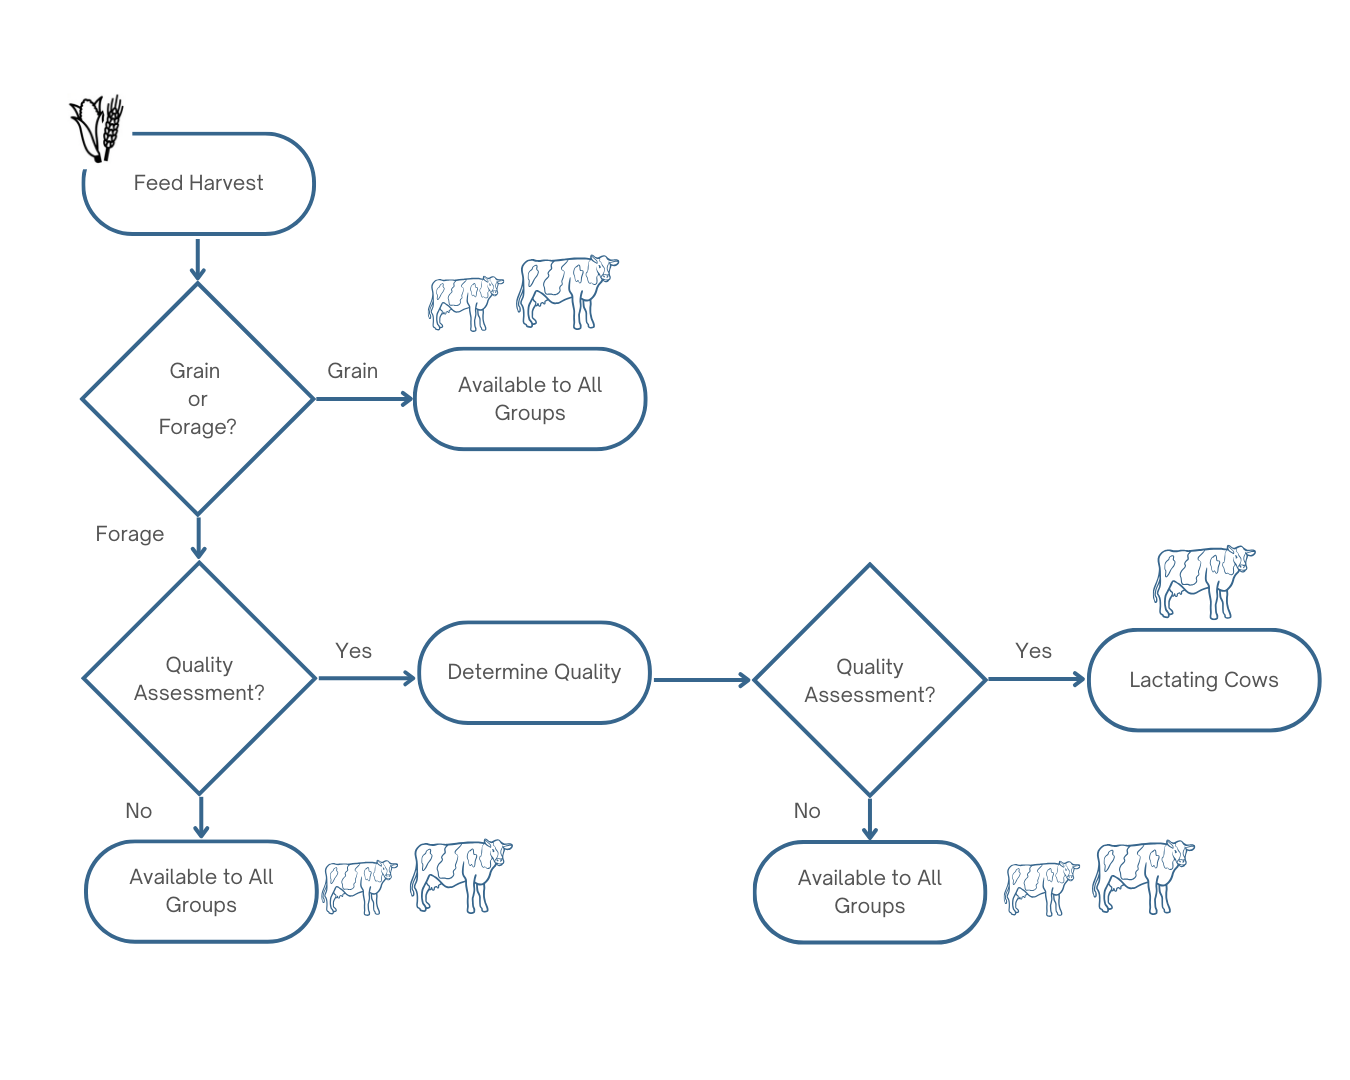
\includegraphics[width=0.9\textwidth]{resources/feedallocation.png} % Replace with your image file
    \caption{Farm grown feed allocation to cattle groups }
    \label{fig:example}
    \end{figure}


We currently represent the quality assessment for the feeds based on a single differentiating nutrient composition value. The differentiating nutrient and levels of the nutrient are given in the feed library.

The feed library that includes both NRC and NASEM feeds does not have feed quality embedded in the feed IDs. Instead, a quality assessment should be made independent of the feed ID number and added as an additional attribute of the stored feed. 

\section{Feed Storage Inputs}
Farmgrown feeds have storage inputs that are described in depth below and consist of the following:
\begin{itemize}
    \item storage classification The class of storage: Grain, Hay, Silage, Baleage.
    \item name  Each storage has a unique name. Ex. "alfalfa\_silage\_storage\_1"
    \item crop\_name The name of the crop being stored.
    \item field\_name    The name of the field the crop was grown in.
    \item storage\_type  The sub-type of the storage class. Ex. "Dry" for grain storage
    \item dm\_loss\_coefficient An input used for grain storages that specifies a loss of DM. Ex. "0.01",
    \item initial\_storage\_dry\_matter The dry matter content upon receipt by the feed storage module.
    \item post\_wilting\_moisture\_percentage The DM content of silage or baleage after wilting.
    \item target\_dry\_matter The final DM content of hay.
    \item additional\_dry\_matter\_loss\_coefficient An optional input to represent DM loss in excess of normal processes.
    \item bale\_size An input used for baleage to specify the diameter of the bale in meters.
    \item rufas\_id The RuFaS feed ID of the stored crop.
    \item capacity 1e10 The maximum mass capacity of the storage.
\end{itemize}

\section{Storage Classifications}
The agricultural production of harvested animal feed is dependent on season, climate, and farm management. In most cases, this means that feed is produced in large quantities when growing conditions are suitable and must be preserved to meet daily animal feed requirements. Microbial spoilage of wet feed products rapidly degrades their nutritional quality and can harm livestock that consume spoiled feed. Viable, cost-effective methods of preservation depend on the crop type and climate, but practically are limited to drying feed beyond the ability to support microbial growth and fermenting feed in the absence of oxygen to produce acid and reduce pH to inhibit spoilage. Feed Storage functions are primarily based on those in the \href{https://www.ars.usda.gov/northeast-area/up-pa/pswmru/docs/integrated-farm-system-model/}{Integrated Farm Systems Model} but modified to accommodate a daily time-step and remove explicit spatial components.



\subsection{Grain} Grains (e.g., corn, rice, soybeans, and wheat) under 15\% moisture are considered dry grain. Higher moisture grains are considered high-moisture. Field harvested grains are not always sufficiently dry for safe storage (\(<\) 15\% moisture) and supplemental drying is often used to achieve target moisture content. Air-drying is a lower-energy drying method for drying grain to ambient levels that consists of passing ambient air through wet grains via fan. Heated-air drying is higher-energy and faster than air-drying, but can reduce moisture below ambient levels. In practice, DM loss from grains are small and are modeled as a fixed percentage loss of dry matter; 1\% for dry grain, 5\% for high-moisture grain.


    \begin{center}
        \(L\_\{gaseous\}  = M\_i\ cdot 0.01\ tag\)
    \end{center}
        \vspace{0.5cm}
    
            {\raggedleft \textbf{[FS.GRN.1]}\par}
            \vspace{0.5cm}

    \begin{center}
        \(L\_\{gaseous\}  = M\_i\ cdot 0.05\ tag\)
    \end{center}
        \vspace{0.5cm}
    
            {\raggedleft \textbf{[FS.GRN.2]}\par}
            \vspace{0.5cm}
            
High-moisture grain as a feed must be managed (fed, fermented, or dried) quickly for this to be accurate, but that is a well-understood requirement and is not explicitly modeled. Nutritional quality changes are variable, but proportional to DM loss. Nutrient values of finished grain not currently tracked are referenced from the most recent edition of NASEM for use in the Animal Module.

\subsection{Hay} Hay is forage that has been dried with a safe preservation moisture content of 12-15\%. Bale storage conditions are separated into protected and unprotected storage with a total of four storage categories in order of decreasing protection from the elements: protected-indoor, protected-wrapped, protected-tarped, and unprotected-outdoor. Less protected hay storages experience additional losses as compared to the most protected storage (indoor) due to exposure to increased airflow and weather according to the following equation. Baled hay loses DM and quality as a function of storage conditions and its moisture content. Bale density plays a role, but is too complex to model directly and is instead estimated as a function of moisture content.

    \begin{center}
        \(L\_\{gaseous\}  = L\_\{base\} + L\_\{additional\}\ tag\)
    \end{center}
        \vspace{0.5cm}
    
            {\raggedleft \textbf{[FS.HAY.1]}\par}
            \vspace{0.5cm}


\textbf{Where we know that}: \\ L\_\{base\} (kg) is the minimum loss expected from protected-indoor as the sum of DM lost in the first 30 days of storage (L\_\{first 30 days\}, kg) and that lost after 30 days (L\_\{post 30 days\}, kg) in order to capture the differing rates of DM loss before and after the forage has reached its target DM content.

    \begin{center}
        \(L\_\{base\}  =  L\_\{first\ 30\ days\} + L\_\{post\ 30\ days\}\ tag\)
    \end{center}
        \vspace{0.5cm}
    
            {\raggedleft \textbf{[FS.HAY.2]}\par}
            \vspace{0.5cm}

\textbf{Where we know that}: \\ 
    \begin{center}
        \(L\_\{first\ 30\ days\} =  \frac{Q + 2433 \cdot [moisture - \frac{MF(1 - moisture)}{1 - MF}]}{(1 - moisture)(14206 - \frac{2433 \cdot MF}{1 - MF})} \cdot \frac{min(30, d)}{30} \ tag\)
    \end{center}
        \vspace{0.5cm}
    
            {\raggedleft \textbf{[FS.HAY.3]}\par}
            \vspace{0.5cm}

    \begin{center}
        \(Q =  104 \cdot moisture^{2.18} \cdot {b_{density}}^{0.5} + 5.72(moisture^{1.23} \cdot {b_{density}}^{0.94})\ tag\)
    \end{center}
        \vspace{0.25cm}
        \textit{Q is the sensible heat generated in the hay (kJ/kg) based on bale density}
        \vspace{0.5cm}
    
            {\raggedleft \textbf{[FS.HAY.4]}\par}
            \vspace{0.5cm}

    \begin{center}
        \(b\_\{density\} =  100 + 440 \cdot moisture\ tag\)
    \end{center}
        \vspace{0.5cm}
    
            {\raggedleft \textbf{[FS.HAY.5]}\par}
            \vspace{0.5cm}

moisture is the fraction of water mass at time of storage (unitless), MF is the target final moisture percent of hay (percent) as defined by the user (default: 12), and d is the number of days the hay has been stored for. 
\vspace{0.2cm}

And
\vspace{0.5cm}

    \begin{center}
        \(L\_\{post\ 30\ days\} =  0.0001 \cdot max(0, d - 30)\ tag\)
    \end{center}
        \vspace{0.5cm}
    
            {\raggedleft \textbf{[FS.HAY.6]}\par}
            \vspace{0.5cm}

        \begin{center}
        \(L\_\{additional\} =  \sum_{i=1}^{d} l \cdot rain_i \cdot max(0.0, \frac{high_i + low_i}{2}) \cdot \frac{1}{b_{density}} \cdot {b_{size}}^3\ tag\)
    \end{center}
        \vspace{0.5cm}
    
            {\raggedleft \textbf{[FS.HAY.7]}\par}
            \vspace{0.5cm}

        \begin{itemize}
            \item d is the number of days the hay has been stored for, 
            \item i is the day of storage that dry matter loss is being calculated for, 
            \item l is the loss coefficient (unitless) from Table 1; \textbf{[FS.HAY.7]}, 
            \item{rain\_i} is the amount of rain on day i (cm), 
            \item{high\_i} is the high temperature on day i (\(\circ C\)), 
            \item{low\_i} is the low temperature on day (\(\circ C\)), 
            \item{b\_density} is the bale density (kg/\(m^2\)) \textbf{[FS.HAY.5]}, and 
            \item{b\_size} is the diameter of the hay bale (m)

        \end{itemize}
\vspace{0.5cm}

\begin{table}[h!]
\centering
\renewcommand{\arraystretch}{1.3}
\caption{Hay storage types and associated fractional loss coefficients}

\begin{tabular}{@{} C{5cm} C{4cm}  @{}}
\toprule
\textbf{Hay Storage Type} & \textbf{Fractional Loss Coefficient (i)}  \\
\midrule
Protected Wrapped & 0.0000216 \\ 
Protected Tarped & 0.0000108 \\
Unprotected Outdoor  & 0.00006 \\
Protected Indoor  & 0 \\
\bottomrule
\end{tabular}
\end{table}

\vspace{1cm}

        \textit{Cumulative water lost from forages stored as hay is determined by:}
        \vspace{0.2cm}

        \begin{center}
        \(M =  F_i \cdot \frac{max(0.0, moisture - MF)}{100} \cdot \frac{min(30, d)}{30}\ tag\)
    \end{center}
        \vspace{0.5cm}
    
            {\raggedleft \textbf{[FS.HAY.8]}\par}
            \vspace{0.5cm}

The lowest energy method for hay drying is passive drying in the field when conditions are suitable, but, similarly to grains, hay can receive supplemental drying via ambient or heated air.  DM loss from protected, baled hay is preferentially from starch and water soluble carbohydrates (60\%), and CP (40\%) which, over time, leads to a proportional increase in NDF and a minor increase in CP over time. Unprotected bales experience increased proportional CP loss (50\% of protected bale DM loss) due to leaching and an additional 17\% loss of NDF dry matter compared to protected bales. Fractional loss coefficients for hay are defined by Table 2:
\vspace{0.5cm}

\begin{table}[h!]
\centering
\renewcommand{\arraystretch}{1.3}
\caption{Protected and unprotected storage, nutrients, and associated fractional loss coefficients}

\begin{tabular}{@{} L{5cm} L{4cm} L{3cm} @{}}
\toprule
\textbf{Hay Storage Type} & \textbf{Nutrient} & \textbf{Fractional Loss Coefficient}  \\
\midrule

\multirow{3}{*}{Unprotected Hay} & Acid Detergent Fiber & 0.0 \\
                           & Neutral Detergent Fiber & 0.17 \\
                           & Crude Protein & 0.4 \\
\multirow{3}{*}{Protected or Indoor Hay} & Acid Detergent Fiber & 0.0 \\
                           & Neutral Detergent Fiber & 0.0 \\
                           & Crude Protein & 0.0 \\
                           
                           
\bottomrule
\end{tabular}
\end{table}
\vspace{1cm}


\subsection{Silage} Silage is the product of anaerobic acidification of non-dry forage, a process called ensiling, and has traditionally been produced as a method of animal feed preservation viable in wet, cool climates where forage production cannot sustain livestock year-round and drying hay at the required scale is challenging \parencite{pahlow2003microbiology}. Typically, forage fermentation is the product of lactic acid bacteria (LAB) consuming WSC present in harvested forage and metabolizing it to a mix of organic products, including the desirable lactic and acetic acids, as well as \(CO_2\) and ethanol. A well-preserved silage relies on a rapid fermentation for retention of optimal feed quality because insufficient or slow acidification is associated with prolonged proteolytic activity, additional dry matter loss, and increased risk of spoilage. \parencite{pahlow2003microbiology, muck2013recent}.

Fermented forages experience DM loss and nutrient changes post-harvest, during fermentation, and during storage. Wilting losses are not currently modeled.


Alfalfa fermentation daily dry matter loss (fraction) is calculated with the equation:


        \begin{center}
        \(L\_{fermentation} = \sum_{i=1}^{d} drymass_{i-1} \cdot (0.00052 - 0.001213(dryfrac_{i-1} - 0.2))\ tag\)
    \end{center}
        \vspace{0.5cm}
    
            {\raggedleft \textbf{[FS.SIL.1]}\par}
        \vspace{0.5cm}

        \begin{itemize}
            \item d is the number of days the alfalfa has been ensiled for, 
            \item i is the day since ensiling that dry matter loss is being calculated for, 
            \item drymass\_{i-1} is the dry matter mass of ensiled alfalfa on day i-1,
            \item dryfrac\_{i-1} is the fraction of ensiled alfalfa fresh mass that is dry matter on day i-1. 
            \item When i is 1, drymass\_{i-1} is the initial amount of ensiled alfalfa dry mass and 
            \item dryfrac\_{i-1} is the initial dry matter fraction of the ensiled alfalfa. This equation is only appropriate for use if dryfrac\_{i-1} is in the range [0.2, 0.6] and the average temperature on day 
            \item i is in the range [5, 45] (\(\circ C\)).
        \end{itemize}
        \vspace{0.5cm}
        
Corn, grass, and small grain daily dry matter loss (fraction) is calculated with the equation:
\vspace{0.2cm}

        \begin{center}
        \(L_{fermentation} = \sum_{i=1}^{d} drymass_{i-1} \cdot (0.000288 - 0.000643(dryfrac_{i-1} - 0.15))\ tag\)
    \end{center}
        \vspace{0.5cm}
    
            {\raggedleft \textbf{[FS.SIL.2]}\par}
        \vspace{0.5cm}

        \begin{itemize}
            \item d is the number of days the forage has been ensiled for, 
            \item i is the day since ensiling that dry matter loss is being calculated for, 
            \item drymass\_{i-1} is the dry matter mass of ensiled forage on day i-1,
            \item dryfrac\_{i-1} is the fraction of ensiled forage fresh mass that is dry matter on day i-1. 
            \item When i is 1, drymass\_{i-1} is the initial amount of ensiled forage dry mass and 
            \item dryfrac\_{i-1} is the initial dry matter fraction of the ensiled forage. This equation is only appropriate for use if dryfrac\_{i-1} is in the range [0.15, 0.6] and the average temperature on day i is in the range [0, 40] (\(\circ C\)).
        \end{itemize}

\begin{table}[h!]
\centering
\renewcommand{\arraystretch}{1.3}
\caption{Silage and the fractional loss coefficients}

\begin{tabular}{@{} L{5cm} L{4cm} L{3cm} @{}}
\toprule
\textbf{Nutrient} & \textbf{Fractional Loss Coefficient}  \\
\midrule

Acid Detergent Fiber & 0.0 \\
Neutral Detergent Fiber & 0.0 \\
Crude Protein & 0.0 \\
                           
                         
\bottomrule
\end{tabular}
\end{table}
\vspace{1CM}

Ensiled crops may also lose dry matter through effluent efflux. Crops that are ensiled with a dry matter content less than 30\% lose both water and dry matter according to the following equations:
\vspace{0.25CM}

        \begin{center}
        \(L_{effluent} = dryfrac\_\{effluent\} \cdot M\_\{effluent\} \cdot 0.1 \cdot max(10, d)\ tag\)
    \end{center}
        \vspace{0.5cm}
    
            {\raggedleft \textbf{[FS.SIL.4]}\par}
        \vspace{0.5cm}
        
\textbf{Where we know that}: \\ 
\vspace{0.2cm}

\(dryfrac_{effluent}\) is the fraction of dry matter in the effluent that is lost, \(M_{effluent}\) is the estimated maximum effluent (kg), and d is the number of days the crop has been ensiled for.
\vspace{0.5cm}

        \begin{center}
        \(ML\_\{effluent\} = (1 - dryfrac_{effluent}) \cdot M_{effluent} \cdot 0.1 \cdot max(10, d) \ tag\)
        \end{center}
        \vspace{0.5cm}
    
            {\raggedleft \textbf{[FS.SIL.5]}\par}
        \vspace{0.5cm}

\textbf{Where we know that:} dryfrac\_{effluent} is the fraction of dry matter in the effluent that is lost,
        \vspace{0.2cm}

M\_{effluent} is the estimated maximum effluent (kg), and d is the number of days the crop has been ensiled for. The fraction of dry matter in effluent is a constant defined as: 
\vspace{0.2cm}

        \begin{center}
        \(dryfrac_{effluent} = 0.1035\ tag\)
    \end{center}
        \vspace{0.5cm}
    
            {\raggedleft \textbf{[FS.SIL.6]}\par}
        \vspace{0.5cm}
        
        \begin{center}
        \(M_{effluent} = mass_{fresh} \cdot ((1 - dryfrac) - 0.7) \ tag\)
    \end{center}
        \vspace{0.5cm}
    
            {\raggedleft \textbf{[FS.SIL.7]}\par}
        \vspace{0.5cm}


\textbf{Where we know that}: \\ \(mass_{fresh}\) is the fresh mass of the crop when it is ensiled (kg) and 
\(dryfrac\) is the fraction of the crop’s fresh mass which is dry matter when it is ensiled.
\vspace{0.2cm}

Dry matter lost in effluent is preferentially from CP, water soluble carbohydrates, and non-protein nitrogen each of which is recalculated by the following equations:
\vspace{0.2cm}

Percent crude protein is calculated as:
\vspace{0.2cm}
        
        \begin{center}
        \(CP_{updated} = \frac{CP_{initial} \cdot 0.01 - 0.3 \cdot DL_{fraction}}{1 - DL_{fraction}} \cdot 100 \ tag\)
    \end{center}
        \vspace{0.5cm}
    
            {\raggedleft \textbf{[FS.SIL.8]}\par}
        \vspace{0.5cm}

\textbf{Where we know that}: \\ \(CP_{initial}\) is the percentage of dry matter mass that is crude protein in the ensiled crop before accounting for dry matter loss to effluent and \(DL_{fraction}\) is the fraction of dry matter mass lost to effluent. The percentage of crude protein is lower-bounded at 0.
\vspace{0.2cm}

The percentage of NPN is calculated with the equation:
\vspace{0.2cm}

        \begin{center}
        \(NPN_{updated} = \frac{(NPN_{initial} \cdot 0.01) \cdot (CP_{initial} \cdot 0.01) - 0.3 \cdot DL_{fraction}}{(CP_{initial} \cdot 0.01) - DL_{fraction}} \cdot 100 \ tag\)
    \end{center}
        \vspace{0.5cm}
    
            {\raggedleft \textbf{[FS.SIL.9]}\par}
        \vspace{0.5cm}


\textbf{Where we know that}: \\ \(NPN_{initial}\) is percentage of dry matter mass that is non-protein nitrogen in the ensiled crop before accounting for dry matter loss to effluent, \(CP_{initial}\) is the percentage of dry matter mass that is crude protein before accounting for dry matter loss to effluent, and \(DL_{fraction}\) is the fraction of dry matter mass lost to effluent. The percentage of non-protein nitrogen is lower-bounded at 0. 
\vspace{0.2cm}

\(DL_{fraction}\) is calculated with the equation:
        \begin{center}
        \(DL_{fraction} = \frac{DM_{lost}}{DM_{initial}}\ tag\)
    \end{center}
        \vspace{0.5cm}
    
            {\raggedleft \textbf{[FS.SIL.10]}\par}
        \vspace{0.5cm}

\textbf{Where we know that}: \\ DM\_lost is the amount of dry matter mass in the ensiled crop after accounting for dry matter lost to effluent, and DM\_initial is the amount of dry matter mass in the ensiled crop before accounting for dry matter lost to effluent.

\subsection{Baleage}
Baleage is an ensiled forage with a DM content between 50-65\% that is baled and wrapped to allow ensiling. The higher DM content of baleage lowers the amount of acid needed to achieve effective preservation and allows it to be consolidated into a bale. Fermentation DM losses for baleage are calculated by \textbf{[FS.SIL.1]} and \textbf{[FS.SIL.2]} with fractional nutrient loss coefficients from Table 3. Baleage does not experience effluent losses.

\subsection{Nutrient Composition}
Changes in dry matter and moisture of stored feed often alter their total and fractional nutrient composition. Recalculating nutrient fractions of stored feeds uses the following equation:
\vspace{0.2cm}

        \begin{center}
        \(n_{updated} = \frac{max(0, \frac{n_{initial}}{100} - C) \cdot DL_{fraction}}{1 - DL_{fraction}} \cdot 100 \ tag\)
    \end{center}
        \vspace{0.5cm}
    
            {\raggedleft \textbf{[FS.NUT.1]}\par}
        \vspace{0.5cm}

\textbf{Where we know that}: \\ n\_updated is the percentage of the target nutrient in the stored crop’s dry matter mass after accounting for dry matter loss, n\_initial is the percentage of the target nutrient in the stored crop’s dry matter mass before accounting for dry matter loss, C is the fractional loss coefficient specific to the nutrient and storage type, and DL\_fraction is the fraction of dry matter lost.
\vspace{0.2cm}

        \begin{center}
        \(DL_{fraction} = \frac{DM_{updated}}{DM_{initial}} \ tag\)
    \end{center}
        \vspace{0.5cm}
    
            {\raggedleft \textbf{[FS.NUT.2]}\par}
        \vspace{0.5cm}





\newpage
\section{Abbreviations}

\renewcommand{\arraystretch}{1.3}
\newcolumntype{L}[1]{>{\raggedright\arraybackslash}p{#1}}

\begin{longtable}{@{} L{4cm} L{12cm} @{}} 
\caption{Common abbreviations used throughout this document} \\

\toprule
\textbf{Abbreviation} & \textbf{Full Term or Phrase} \\
\midrule
\endfirsthead

\multicolumn{2}{@{}l}{\textit{Table continued from previous page}} \\
\toprule
\textbf{Abbreviation} & \textbf{Full Term or Phrase} \\
\midrule
\endhead

\midrule
\multicolumn{2}{@{}r@{}}{\textit{Continued on next page}} \\
\endfoot

\bottomrule
\endlastfoot

ADF & Acid detergent fiber (\% of DM) \\
ADG & Average daily weight gain (g/d) \\
Age1stBred & First breeding age (month) \\
BCS5 & Body condition score (1–5 basis) \\
BW & Body weight (kg) \\
Ca & Calcium content (\% of DM) \\
CBW & Calf birth weight (kg) \\
CI & Calving interval (d) \\
cm & centimeter \\
Cost & Feed cost (\$/kg of DM) \\
CP & Crude protein (\% of DM) \\
d & days \\
DE & Digestible energy (standard value, Mcal/kg) \\
DIM & Days in milk \\
DM & Dry matter (\% of as-fed basis) \\
DMI & Dry matter intake \\
DOP & Days of pregnancy (d) \\
dRUP & RUP degradability (\% of RUP) \\
EE & Ether extract, in crude fat (\% DM) \\
EndCP & Endogenous CP \\
EndN & Endogenous N \\
EQSBW & Equivalent shrunk body weight (kg) \\
FA & Fatty acids \\
FIPS & Federal Information Processing Standards \\
g & grams \\
GE & Gross energy (standard value, Mcal/kg) \\
GrUterW & Gravid uterine weight (kg) \\
Kd & Rumen protein degradation rate (\%/h) \\
kg & kilograms \\
kJ & kilojoule \\
L & liters \\
m & meter \\
max & maximum \\
Mcal & Megacalorie \\
MCP & Microbial Crude Protein \\
ME & Metabolizable energy (standard value, Mcal/kg) \\
MICP & Microbial CP \\
min & minimum \\
mL & milliliters \\
MN & Microbial N \\
MP & Metabolizable protein \\
MTP & Microbial TP \\
MW & Mature body weight (kg) \\
MY & Milk yield \\
N & Nitrogen (\% of DM) \\
NASEM & National Academies of Sciences, Engineering, and Medicine \\
NDF & Neutral detergent fiber (\% of DM) \\
NEG & Net energy for growth (standard value, Mcal/kg) \\
NEL & Net energy for lactation (standard value, Mcal/kg) \\
NEM & Net energy for maintenance (standard value, Mcal/kg) \\
nNDF & Nondigestible Neutral Detergent Fiber \\
NPN & Non-protein Nitrogen \\
NRC & National Research Council (updated in 2021 to NASEM) \\
OM & Organic matter (\% of DM) \\
P & Phosphorus content (\% of DM) \\
PAF & Processing adjustment factor (not used) \\
Parity & Number of lactations \\
PrevTemp & Average daily temperature of last month (°C) \\
RDP & Ruminally degraded CP \\
ROM & Residual OM (\% of DM) \\
RUP & Ruminally undegraded CP \\
s & seconds \\
TAN & Total ammoniacal N \\
TDN & Total digestible nutrient (\% of DM) \\
TP & True protein (\% of DM) \\
USDA & United States Department of Agriculture \\
UterW & Uterine weight (kg) \\
WSC & Water Soluble Carbohydrates \\
\end{longtable}


\newpage
\section{References}
\printbibliography[heading=subbibliography,title={Feed Storage Module}]
\end{refsection}


\end{document}


\end{document}
